%
% tikztemplate.tex
%
% (c) 2018 Prof Dr Andreas Müller, Hochschule Rapperswil
%
\documentclass[tikz,12pt]{standalone}
\usepackage{times}
\usepackage{amsmath}
\usepackage{txfonts}
\usepackage[utf8]{inputenc}
\usepackage{graphics}
\usepackage{color}
\usepackage{pifont}
\usetikzlibrary{arrows,intersections,math,calc}
\begin{document}

\def\punkt#1{
        \fill[color=white] #1 circle[radius=0.08];
        \draw #1 circle[radius=0.08];
}

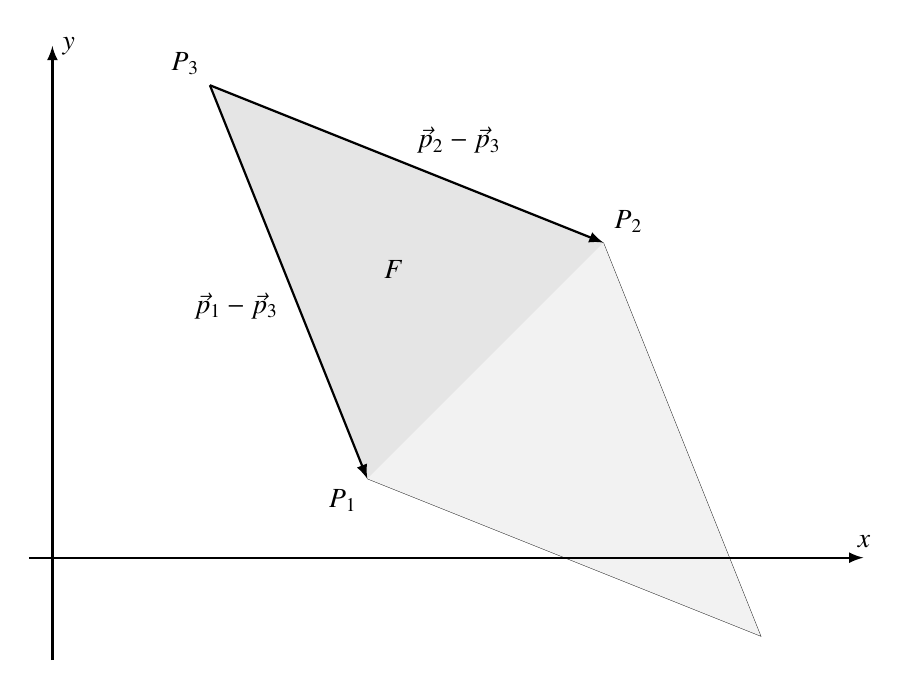
\begin{tikzpicture}[>=latex,thick]

\coordinate (O) at (0,0);
\coordinate (P1) at (4,1);
\coordinate (P2) at (7,4);
\coordinate (P3) at (2,6);
\coordinate (P4) at ($(P2)+(P1)-(P3)$);

\fill[color=gray!20] (P3)--(P1)--(P2)--cycle;
\fill[color=gray!10] (P1)--(P4)--(P2)--cycle;

\draw[line width=0.1pt] (P1)--(P4)--(P2);

\draw[->] (P3)--(P1);
\draw[->] (P3)--(P2);

\punkt{(P1)} \node at (P1) [below left] {$P_1$};
\punkt{(P2)} \node at (P2) [above right] {$P_2$};
\punkt{(P3)} \node at (P3) [above left] {$P_3$};

\node at ($0.5*(P3)+0.5*(P2)$) [above right] {$\vec{p}_2-\vec{p}_3$};
\node at ($0.5*(P3)+0.5*(P1)$) [below left] {$\vec{p}_1-\vec{p}_3$};

\draw[->] (-0.3,0)--(10.3,0) coordinate[label={$x$}];
\draw[->] (0,-1.3)--(0,6.5) coordinate[label={right:$y$}];

\node at ($0.333*(P1)+0.333*(P2)+0.333*(P3)$) {$F$};

\end{tikzpicture}

\end{document}

